\section{Study 1 --- Sovereignty Scoring}
\label{sec:method-study1}

This study uses the Cloud Sovereignty Framework published by the European
Commission \cite{EC_DIGIT_CloudSovereignty_2025}, for the reasons given in
\cref{subsec:definition-adopted}. The framework was adopted rather than designed
here, so what follows describes how it was applied.

The framework has three parts: a scale of five assurance levels, eight weighted
objectives, and for each objective a list of contributing factors.

\subsection*{The five assurance levels}

The framework treats sovereignty as a degree rather than a yes or no, and
measures it on a scale of five levels. It calls them Sovereignty Effectiveness
Assurance Levels, or seals. \Cref{tab:seal-levels} gives them.

\begin{table}[htbp]
  \centering
  \caption{The five assurance levels, as defined by the framework
           \cite{EC_DIGIT_CloudSovereignty_2025}.}
  \label{tab:seal-levels}
  \small
  \renewcommand{\arraystretch}{1.3}
  \begin{tabularx}{\textwidth}{@{}l l X@{}}
    \toprule
    \textbf{Level} & \textbf{Name} & \textbf{Meaning} \\
    \midrule
    SEAL-0 & No sovereignty
      & Service under the exclusive control of non-\acs{EU} parties, governed
        entirely in non-\acs{EU} jurisdictions. \\
    SEAL-1 & Jurisdictional sovereignty
      & \acs{EU} law formally applies but with limited practical
        enforceability; service still under the exclusive control of
        non-\acs{EU} parties. \\
    SEAL-2 & Data sovereignty
      & \acs{EU} law applicable and enforceable, with material non-\acs{EU}
        dependencies remaining; service under their indirect control. \\
    SEAL-3 & Digital resilience
      & \acs{EU} law applicable and enforceable, with \acs{EU} actors
        exercising meaningful but not full influence; service under only
        marginal non-\acs{EU} control. \\
    SEAL-4 & Full digital sovereignty
      & Technology and operations under complete \acs{EU} control, subject only
        to \acs{EU} law, with no critical non-\acs{EU} dependencies. \\
    \bottomrule
  \end{tabularx}
\end{table}

The scale is built around one question asked five times over: how much control
does a party outside the Union still hold? At SEAL-1 that control is exclusive,
at SEAL-2 indirect, at SEAL-3 marginal, and at SEAL-4 absent. European law
becoming applicable is not the same as European actors being in charge, and the
scale separates the two.

\subsection*{The eight objectives}

The framework divides sovereignty into eight objectives, each carrying a weight.
\Cref{tab:sov-objectives} lists them.

\begin{table}[htbp]
  \centering
  \caption{The eight sovereignty objectives. The weights are the framework's;
           the number of questions and the minimum seal were set for this study.}
  \label{tab:sov-objectives}
  \small
  \begin{tabularx}{\textwidth}{@{}l X r r r@{}}
    \toprule
    & \textbf{Objective} & \textbf{Weight} & \textbf{Questions} & \textbf{Minimum} \\
    \midrule
    SOV-1 & Strategic sovereignty      & 15\,\% & 6 & 3 \\
    SOV-2 & Legal and jurisdictional   & 10\,\% & 5 & 4 \\
    SOV-3 & Data and AI sovereignty    & 10\,\% & 5 & 3 \\
    SOV-4 & Operational sovereignty    & 15\,\% & 6 & 2 \\
    SOV-5 & Supply chain               & 20\,\% & 5 & 2 \\
    SOV-6 & Technology                 & 15\,\% & 4 & 2 \\
    SOV-7 & Security and compliance    & 10\,\% & 6 & 3 \\
    SOV-8 & Environmental              &  5\,\% & 4 & 1 \\
    \midrule
    & \textbf{Total}                   & \textbf{100\,\%} & \textbf{41} & \\
    \bottomrule
  \end{tabularx}
\end{table}

Two things in that table shape the results. Supply chain carries the heaviest
weight of the eight, which matches the argument in \cref{sec:full-stack} that
sovereignty claimed at one layer depends on the layers beneath it. And the legal
objective carries the highest minimum: a provider has to reach the top level
there to pass at all, however well it does elsewhere.

The weights are the framework's. The minimum seal on each objective is set by
whoever runs the procurement, and the levels in the last column were set for this
study.

\subsection*{The contributing factors, as questions}

Each objective has a set of contributing factors, listed in the framework. Each
factor was written as a question that can be answered from a provider's published
documentation. \Cref{tab:sov-questions-a,tab:sov-questions-b} give the forty-one
questions, abbreviated. Each was answered for each provider from published
sources.

\begin{table}[htbp]
  \centering
  \caption{Assessment questions, SOV-1 to SOV-4.}
  \label{tab:sov-questions-a}
  \footnotesize
  \renewcommand{\arraystretch}{1.2}
  \begin{tabularx}{\textwidth}{@{}c X X X X@{}}
    \toprule
    & \textbf{SOV-1}\newline Strategic
    & \textbf{SOV-2}\newline Legal
    & \textbf{SOV-3}\newline Data \& AI
    & \textbf{SOV-4}\newline Operational \\
    \midrule
    Q1 & Decisive authority within the \acs{EU}?
       & Governed only by member-state law?
       & Customer holds the encryption keys?
       & Workloads movable without lock-in? \\
    Q2 & Protected against non-\acs{EU} takeover?
       & Free of extraterritorial laws?
       & Access to data and \acs{AI} auditable?
       & \acs{EU} operators can run it alone? \\
    Q3 & Financed from within the \acs{EU}?
       & No channel for compelled access?
       & Deletion verifiable and irreversible?
       & \acs{EU} talent pool exists? \\
    Q4 & Invests and employs in the \acs{EU}?
       & Free of export-control regimes?
       & Storage and processing \acs{EU}-only?
       & Support delivered from the \acs{EU}? \\
    Q5 & Active in \acs{EU} sovereignty work?
       & Intellectual property \acs{EU}-owned?
       & \acs{AI} models governed in the \acs{EU}?
       & Documentation and source available? \\
    Q6 & Survives withdrawal of vendor support?
       & ---
       & ---
       & Subcontractors under \acs{EU} law? \\
    \bottomrule
  \end{tabularx}
\end{table}

\begin{table}[htbp]
  \centering
  \caption{Assessment questions, SOV-5 to SOV-8.}
  \label{tab:sov-questions-b}
  \footnotesize
  \renewcommand{\arraystretch}{1.2}
  \begin{tabularx}{\textwidth}{@{}c X X X X@{}}
    \toprule
    & \textbf{SOV-5}\newline Supply chain
    & \textbf{SOV-6}\newline Technology
    & \textbf{SOV-7}\newline Security
    & \textbf{SOV-8}\newline Environmental \\
    \midrule
    Q1 & Hardware made in trusted jurisdictions?
       & Open standards and documented \acsp{API}?
       & Holds recognised \acs{EU} certifications?
       & Energy-efficient, with published targets? \\
    Q2 & Firmware of \acs{EU} origin?
       & Stack open-source and modifiable?
       & Compliant with \acs{GDPR}, \acs{NIS2}, \acs{DORA}?
       & Circular practices for hardware? \\
    Q3 & Software built and updated in the \acs{EU}?
       & Architecture and dependencies disclosed?
       & Security operations under \acs{EU} law?
       & Carbon and water use published? \\
    Q4 & Free of reliance on non-\acs{EU} vendors?
       & Free of non-\acs{EU} \acs{HPC} silicon?
       & Customer oversight of monitoring?
       & Renewable or low-carbon energy? \\
    Q5 & Supply chain auditable end to end?
       & ---
       & \acs{EU}-compliant breach reporting?
       & --- \\
    Q6 & ---
       & ---
       & Independent audits permitted?
       & --- \\
    \bottomrule
  \end{tabularx}
\end{table}

\subsection*{The verdicts}

Each question takes one of three verdicts:

\begin{itemize}
  \item \textbf{Yes (Y)} --- the provider meets the condition, and a published
        document shows it. Two points.
  \item \textbf{Partly (P)} --- the provider meets it in part, but not fully. Or
        no published document shows it. One point.
  \item \textbf{No (N)} --- the provider does not meet it. No points.
\end{itemize}

\subsection*{From verdicts to a score}

The verdicts on an objective are added together and expressed as a share of the
points available. Writing $Q_n$ for the questions belonging to objective $n$ and
$v(q)$ for the points a verdict is worth:

\begin{equation}
  \label{eq:sov-share}
  r_n = \frac{\displaystyle\sum_{q \in Q_n} v(q)}{2\,\lvert Q_n \rvert}
\end{equation}

The denominator is two points for every question, so $r_n$ runs from 0 to 1.
That share is divided into five equal bands of twenty percentage points, which
gives the seal reached on that objective:

\begin{equation}
  \label{eq:sov-seal}
  \text{seal}_n =
  \begin{cases}
    0 & r_n \le 0.20\\
    1 & 0.20 < r_n \le 0.40\\
    2 & 0.40 < r_n \le 0.60\\
    3 & 0.60 < r_n \le 0.80\\
    4 & r_n > 0.80
  \end{cases}
\end{equation}

The overall score combines the eight seals in proportion to their weights, and is
reported on a scale of 0 to 100. Dividing a seal by four, the highest level,
gives the fraction of full sovereignty reached on that objective; the weight
$w_n$ sets how much that objective contributes.

\begin{equation}
  \label{eq:sov-score}
  S_{\text{sov}} = \sum_{n=1}^{8} \frac{\text{seal}_n}{4} \times w_n \times 100
\end{equation}

The score is not the only result. A provider also passes or fails, and it passes
only if every objective reaches its own minimum $m_n$:

\begin{equation}
  \label{eq:sov-pass}
  \text{pass} \iff \text{seal}_n \ge m_n \quad \text{for every } n = 1,\ldots,8
\end{equation}

Worked through: the legal objective has five questions, so ten points are
available. Two yes, two partly and one no earns six points, a share of 0.60,
which gives SEAL-2 and contributes five points to the total. The minimum on that
objective is SEAL-4, so the provider fails it.

The two outcomes can disagree: a provider may score well overall and still fail
because a single objective falls short. That is deliberate, and it is the rule
from \cref{ch:methodology} applied within a single study --- a weakness in one
place is not made good by strength in another.

The minimum levels are settings rather than fixed rules. They can be raised or
lowered and the assessment recomputed, which is how the sensitivity analysis in
\cref{subsec:sensitivity} is carried out.

\subsection*{What the method produces}

Applying the instrument to the eighteen providers gives a level on each of the
eight objectives, and from those an overall score. \Cref{tab:sov-seals} shows the
levels. Shaded cells are those below the minimum for that objective; a provider
passes only if none of its cells is shaded.

\begin{table}[htbp]
  \centering
  \caption{Level reached by each provider on each objective. Shaded cells fall
           below the minimum required, shown in the second header row.}
  \label{tab:sov-seals}
  \small
  \renewcommand{\arraystretch}{1.35}
  \begin{tabularx}{\textwidth}{@{}l *{8}{>{\centering\arraybackslash}X} r c@{}}
    \toprule
    \textbf{Provider}
    & \textbf{SOV}\newline\textbf{1} & \textbf{SOV}\newline\textbf{2}
    & \textbf{SOV}\newline\textbf{3} & \textbf{SOV}\newline\textbf{4}
    & \textbf{SOV}\newline\textbf{5} & \textbf{SOV}\newline\textbf{6}
    & \textbf{SOV}\newline\textbf{7} & \textbf{SOV}\newline\textbf{8}
    & \textbf{Score} & \textbf{Pass} \\
    \textit{minimum seal}
    & 3 & 4 & 3 & 2 & 2 & 2 & 3 & 1 & & \\
    \midrule
    STACKIT        & 4 & 4 & 3 & 4 & 2 & 3 & 4 & 3 & 82.5 & \checkmark \\
    Cyso Cloud     & 3 & 4 & 3 & 4 & 2 & 3 & 4 & 3 & 78.8 & \checkmark \\
    noris network  & 4 & 4 & 3 & 4 & \cellcolor{black!12}1 & 3 & 4 & 3 & 77.5 & --- \\
    Cleura         & 3 & 4 & 3 & 4 & 2 & 3 & 3 & 3 & 76.2 & \checkmark \\
    Elastx         & 3 & 4 & 3 & 4 & 2 & 3 & 3 & 3 & 76.2 & \checkmark \\
    Hetzner        & 4 & 4 & \cellcolor{black!12}2 & 4 & 2 & 2 & 3 & 4 & 75.0 & --- \\
    Scaleway       & 4 & \cellcolor{black!12}3 & 4 & 4 & \cellcolor{black!12}1 & 2 & 3 & 4 & 72.5 & --- \\
    plusserver     & 3 & 4 & 3 & 3 & 2 & 2 & 4 & 3 & 71.2 & \checkmark \\
    Exoscale       & \cellcolor{black!12}2 & \cellcolor{black!12}3 & 3 & 4 & 2 & 2 & 4 & 2 & 67.5 & --- \\
    T-Cloud Public & 4 & \cellcolor{black!12}2 & 3 & 3 & \cellcolor{black!12}1 & 2 & 4 & 4 & 66.2 & --- \\
    Infomaniak     & 3 & \cellcolor{black!12}2 & \cellcolor{black!12}2 & 3 & \cellcolor{black!12}1 & 3 & 3 & 4 & 61.3 & --- \\
    UpCloud        & 3 & \cellcolor{black!12}3 & \cellcolor{black!12}2 & 4 & \cellcolor{black!12}1 & 2 & 3 & 2 & 61.3 & --- \\
    OVHcloud       & 3 & \cellcolor{black!12}1 & \cellcolor{black!12}2 & 3 & 2 & 2 & 3 & 3 & 58.8 & --- \\
    nine           & \cellcolor{black!12}2 & \cellcolor{black!12}2 & \cellcolor{black!12}2 & 3 & \cellcolor{black!12}1 & 3 & 3 & 3 & 56.2 & --- \\
    IONOS          & \cellcolor{black!12}2 & \cellcolor{black!12}2 & \cellcolor{black!12}2 & 3 & \cellcolor{black!12}1 & 2 & 3 & 3 & 52.5 & --- \\
    Locally hosted & \cellcolor{black!12}2 & 4 & 3 & 2 & \cellcolor{black!12}1 & 2 & \cellcolor{black!12}2 & 1 & 51.3 & --- \\
    Arvato Systems & 3 & \cellcolor{black!12}2 & \cellcolor{black!12}2 & 2 & \cellcolor{black!12}1 & \cellcolor{black!12}1 & 4 & 3 & 51.2 & --- \\
    T-Systems OTC  & \cellcolor{black!12}2 & \cellcolor{black!12}1 & 3 & 2 & \cellcolor{black!12}0 & 2 & 4 & 3 & 46.2 & --- \\
    \bottomrule
  \end{tabularx}
\end{table}

Reading down the columns shows where the difficulty lies. Two objectives account
for almost all the shading. Ten of the eighteen fall short on SOV-2, the legal
objective, where the framework demands the highest level of the eight. Ten also
fall short on SOV-5, supply chain --- but there the requirement is one of the
lowest, and no provider in the set reaches above level~2 on it at all.

The two failures are not the same kind of problem. A provider can improve its
legal position by restructuring or by contract. It cannot improve its
supply-chain position the same way, because the hardware and firmware it runs on
are not made in Europe. This is the constraint described in \cref{sec:full-stack}
appearing in the measurements, and it explains why the objective carrying the
heaviest weight is also the one on which every provider does worst.

The remaining objectives are cleared almost universally: operational sovereignty
and environmental performance by all eighteen, technology and security by all but
one each.

Combining the eight levels by weight gives the overall score.
\Cref{fig:sov-ranking} ranks the providers by it, marking those that clear every
minimum.

\begin{figure}[htbp]
  \centering
  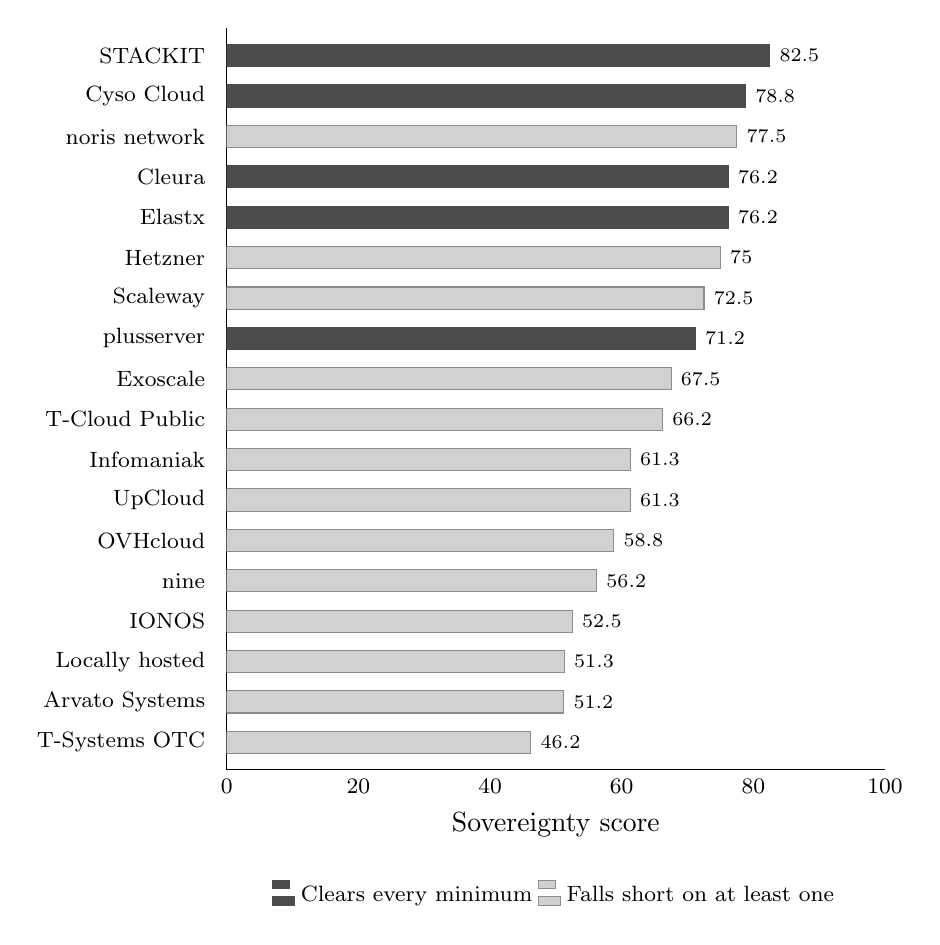
\begin{tikzpicture}
    \begin{axis}[
      xbar,
      width=0.82\textwidth, height=11cm,
      xmin=0, xmax=100,
      xlabel={Sovereignty score},
      bar width=8pt,
      enlarge y limits=0.04,
      symbolic y coords={{T-Systems OTC},{Arvato Systems},{Locally hosted},
                         {IONOS},{nine},{OVHcloud},{UpCloud},{Infomaniak},
                         {T-Cloud Public},{Exoscale},{plusserver},{Scaleway},
                         {Hetzner},{Elastx},{Cleura},{noris network},
                         {Cyso Cloud},{STACKIT}},
      ytick={{T-Systems OTC},{Arvato Systems},{Locally hosted},{IONOS},
             {nine},{OVHcloud},{UpCloud},{Infomaniak},{T-Cloud Public},
             {Exoscale},{plusserver},{Scaleway},{Hetzner},{Elastx},
             {Cleura},{noris network},{Cyso Cloud},{STACKIT}},
      yticklabel style={font=\footnotesize},
      xticklabel style={font=\footnotesize},
      nodes near coords,
      nodes near coords style={font=\scriptsize, text=black},
      legend style={at={(0.5,-0.14)}, anchor=north, legend columns=2,
                    font=\footnotesize, draw=none},
      tick style={draw=none},
      axis x line*=bottom, axis y line*=left,
    ]
      \addplot[xbar, bar shift=0pt, fill=black!70, draw=black!70]
        coordinates {(71.2,{plusserver}) (76.2,{Elastx}) (76.2,{Cleura})
                     (78.8,{Cyso Cloud}) (82.5,{STACKIT})};
      \addplot[xbar, bar shift=0pt, fill=black!18, draw=black!45]
        coordinates {(46.2,{T-Systems OTC}) (51.2,{Arvato Systems})
                     (51.3,{Locally hosted}) (52.5,{IONOS}) (56.2,{nine})
                     (58.8,{OVHcloud}) (61.3,{UpCloud}) (61.3,{Infomaniak})
                     (66.2,{T-Cloud Public}) (67.5,{Exoscale})
                     (72.5,{Scaleway}) (75.0,{Hetzner}) (77.5,{noris network})};
      \legend{Clears every minimum, Falls short on at least one}
    \end{axis}
  \end{tikzpicture}
  \caption{Sovereignty scores for the eighteen providers, with those clearing
           every minimum shown in dark.}
  \label{fig:sov-ranking}
\end{figure}

The dark bars are not the top five. Five providers clear every minimum, but three
that score higher than one of them do not: noris network reaches 77.5 and fails
on supply chain, while plusserver passes on 71.2. Ranking by score alone would
place noris network third and plusserver eighth, and would put forward a provider
that does not meet the requirements.

The two Deutsche Telekom entries also separate sharply. T-Cloud Public scores
66.2 against 46.2 for Open Telekom Cloud --- twenty points between two names for
what the company describes as one platform. That difference is examined in
\cref{sec:study1}.
